\chapter{Results \& Discussion}
\label{ch:results}

The following chapter presents the experimental results alongside a discussion 
of the findings. It begins with an overview of the experimental runs, followed 
by selected outcomes from each. First, the performance of the \gls{pd+} controller 
is examined, with step response results shown for heading, roll, and both 
lateral and longitudinal position control. Next, the results from experiments using the 
task-priority controller are presented, focusing initially on the scenario in which the 
robot is stretched. This is followed by results from experiments where the 
robot is bent, utilizing set-based tasks. Finally, a comparison is 
made between runs with and without low-pass filtering of the generalized velocities
and joint angles.


\section{Overview of Results}

Each experimental run is classified by the time it was started, and there are a total
of \(10\) runs that will be presented in the following sections. The format
of the run name is \texttt{MMDD-HHMMSS}, where the first part is the date
and the second part is the time. The raw data collected from experiments can be
downloaded from \cite{githubdata}, along with scripts for generating plots.
An overview of the runs is presented in
\autoref{tab:eelume:experimental-runs}, which includes the run name, the
controller used, if the velocity measurements were low-pass filtered, and a
brief description of each run.

\begin{table}[!ht]
    \centering
    \begin{tabular}{|c|c|c|c|}
        \hline
        Run Name & Controller & Low-pass & Case \\ \hline \hline
        \multirow{2}{*}{0513 - 135042} & \gls{pd+} & No & Heading \\ \cline{2-4}
        & \multicolumn{3}{p{0.75\linewidth}|}{Reference in yaw angle set to \(20\) degrees after 20 seconds.} \\ \hline
        \multirow{2}{*}{0519 - 141406} & \gls{pd+} & No & Roll \\ \cline{2-4}
        & \multicolumn{3}{p{0.75\linewidth}|}{Reference in roll angle set to \(20\) degrees after 20 seconds.} \\ \hline
        \multirow{2}{*}{0519 - 133631} & \gls{pd+} & No & Lateral Position \\ \cline{2-4}
        & \multicolumn{3}{p{0.75\linewidth}|}{Reference in north position set to \(+1\) m after 20 seconds.} \\ \hline
        \multirow{2}{*}{0519 - 134500} & \gls{pd+} & No & Longitudinal Position \\ \cline{2-4}
        & \multicolumn{3}{p{0.75\linewidth}|}{Reference in east position set to \(+1\) m after 20 seconds.} \\ \hline
        \hline
        \multirow{2}{*}{0519 - 141527} & Kinematic-level \gls{tpc} & Yes & Stretch \\ \cline{2-4}
        & \multicolumn{3}{p{0.75\linewidth}|}{Showing case \textit{stretch} with decoupled quaternion gains.} \\ \hline
        %\multirow{2}{*}{0519 - 144113} & Kinematic-level \gls{tpc} & No & Stretch \\ \cline{2-4}
        %& \multicolumn{3}{p{0.75\linewidth}|}{Showing case \textit{stretch} with no compensation term.} \\ \hline
        \hline
        \multirow{2}{*}{0519 - 161629} & Kinematic-Level \gls{tpc} & Yes & Bend \\ \cline{2-4}
        & \multicolumn{3}{p{0.75\linewidth}|}{Showing case \textit{bend}, with compensation term.} \\ \hline
        \multirow{2}{*}{0519 - 161107} & Kinematic-Level \gls{tpc} & No & Bend \\ \cline{2-4}
        & \multicolumn{3}{p{0.75\linewidth}|}{Showing case \textit{bend}, without compensation term.} \\ \hline
        \hline
        \multirow{2}{*}{0513 - 154920} & Kinematic-Level \gls{tpc} & No & Stretch \\ \cline{2-4}
        & \multicolumn{3}{p{0.75\linewidth}|}{Showing case \textit{stretch} with no low-pass filtering.} \\ \hline
        \multirow{2}{*}{0519 - 135739} & Kinematic-Level \gls{tpc} & Yes & Stretch \\ \cline{2-4}
        & \multicolumn{3}{p{0.75\linewidth}|}{Showing case \textit{stretch} with low-pass filtering.} \\ \hline
    \end{tabular}
    \caption[An overview of the experimental runs]{An overview of the experimental
    runs presented in this chapter along with a brief description of each.
    The low-pass column indicates whether or not the generalized velocities and joint measurements were low-pass filtered.}
    \label{tab:eelume:experimental-runs}
\end{table}

% -----------------------------------------------------------------------------
\section{DP-Control}

\paragraph{Experimental setup.}
The first group of experiments aims to show the response of the lower-level \gls{pd+} controller.
Ideally, the lower-level controller should be able to follow a setpoint
in the position, attitude, and joint angles. How fast or slow the controller can follow
the setpoint will have an impact on how high frequency contents the tasks can have:
the better the lower-level controller follows the setpoint, the higher frequency contents
the tasks can have. The lower-level controller is implemented as a \gls{pd+} controller
as described in \autoref{sec:tpc:low_level_control}.

The \(\bm{K}_p\) and \(\bm{K}_d\) matrices of the \gls{pd+} controller are set to
diagonal matrices with the following values:
\begin{subequations}
\begin{align}
    \bm{K}_p &= \operatorname{diag}\left( 50, 160, 120, 2 \frac{180}{\pi}, 20 \frac{180}{\pi}, 22 \frac{180}{\pi}, 10, 10, 10, 10 \right) \\
    \bm{K}_d &= \operatorname{diag}\left( 20, 0, 40, \frac{2}{3} \frac{180}{\pi}, 0, 0, 4, 4, 4, 4 \right)
\end{align}
\end{subequations}
where the units for the first three elements of \(\bm{K}_p\)are in N/m, and the last four are in Nm/deg.
The units for the attitude coefficients are not specified, as they are multiplied by the
vector part of the error quaternion, which is dimensionless. The units for the first three elements
of \(\bm{K}_d\) are in N/(m/s), and the last four are in Nm/(deg/s).

\subsection{Heading Control}

\begin{figure}[!ht]
    \centering
    \includegraphics[width=1.0\textwidth,page=1]{assets/ignored/plots/pd.pdf}
    \caption{Position of Eelume robot during heading control with \gls{pd+} controller.}
    \label{fig:results:dp_heading:pos}
\end{figure}
\begin{figure}[!ht]
    \centering
    \includegraphics[width=1.0\textwidth,page=2]{assets/ignored/plots/20250513-135042.pdf}
    \caption{Generalized velocity of Eelume robot during heading control with \gls{pd+} controller.}
    \label{fig:results:dp_heading:vel}
\end{figure}
\begin{figure}[!ht]
    \centering
    \includegraphics[width=1.0\textwidth,page=5]{assets/ignored/plots/20250513-135042.pdf}
    \caption{Thruster forces and joint motor torques of Eelume robot during heading control with \gls{pd+} controller.}
    \label{fig:results:dp_heading:forces2}
\end{figure}

\paragraph{Results.}
\autoref{fig:results:dp_heading:pos} shows the position and orientation of the 
Eelume robot during a heading control task. The robot is commanded to turn to 
a heading of \(20^\circ\) at \(t = 20\) seconds. The yaw angle gradually 
converges to the reference, with an overshoot of approximately \(3^\circ\), 
followed by damped oscillations. The system settles within a few degrees of 
the reference after approximately \(25\) seconds. The roll and pitch angles 
remain near \(0^\circ\), indicating stable attitude in those directions.

The \gls{ned} position of the robot, which is controlled to remain near the 
origin, is somewhat affected by the heading maneuver. Both the north and down 
positions exhibit a steady-state offset of approximately \(0.3\,\mathrm{m}\) 
from the reference. This suggests a degree of coupling between the heading and 
translational dynamics. The joint angle measurements also show considerable 
high-frequency noise.

The generalized velocities, shown in \autoref{fig:results:dp_heading:vel}, 
further highlight this noise. While the angular velocities are visibly noisy, 
the joint velocities are particularly affected, with high-frequency 
oscillations and spikes reaching up to \(100^\circ/\mathrm{s}\).

\autoref{fig:results:dp_heading:forces2} presents the resulting thruster 
forces and joint motor torques. Although the thruster forces contain some high-
frequency noise, its amplitude is moderate compared to that of the generalized 
velocities. The joint torques, however, exhibit significant noise, frequently 
reaching the actuator limit of \(\pm16\,\mathrm{Nm}\).

\paragraph{Discussion.}

The results in \autoref{fig:results:dp_heading:pos} confirm that the \gls{pd+} 
controller is capable of driving the heading of the Eelume robot to a desired 
value. However, the response is relatively slow, which can be attributed to 
the substantial hydrodynamic forces resisting rotation about the body \(z\)-
axis. The observed overshoot and oscillatory behavior suggest that further 
tuning of the controller gains could improve performance. The robot's large 
inertia around the \(z\)-axis likely contributes to the sluggish response.

An important observation is the degradation in position-holding performance 
during the heading change. This likely results from coupling between the 
degrees of freedom, as the thrusters must simultaneously handle both position 
and heading control.

The joint angle noise, noted in \autoref{fig:results:dp_heading:pos}, aligns 
with the joint velocity spikes observed in \autoref{fig:results:dp_heading:vel
}. These artifacts are consistent with the "jittering" behavior described in
\autoref{sec:experimental_setup:assumptions_and_limitations}. The presence of 
similar high-frequency noise in the thruster forces and joint torques
(\autoref{fig:results:dp_heading:forces2}) can be explained by the unfiltered 
propagation of noisy joint and velocity measurements through the controller 
and thruster allocation algorithms.

Of particular concern is the behavior of the joint motor torques, which 
resemble a "bang-bang" control strategy rather than a smooth \gls{dp} response
. This is partly due to the high proportional gain in the controller—set to
\(10\,\mathrm{Nm}/^\circ\)—meaning that a \(1^\circ\) error induces a 
\(10\,\mathrm{Nm}\) corrective torque. While this gain yields low joint angle 
errors, it also results in aggressive, high-frequency control actions that may 
not be ideal for the mechanical components and actuators. Future work should 
consider the use of low-pass filtering or gain scheduling to mitigate these effects.

\FloatBarrier

% -----------------------------------------------------------------------------
\subsection{Roll Control}

\begin{figure}[!ht]
    \centering
    \includegraphics[width=1.0\textwidth,page=2]{assets/ignored/plots/pd.pdf}
    \caption{Position of Eelume robot during roll control with \gls{pd+} controller.}
    \label{fig:results:dp_roll:pos}
\end{figure}

\paragraph{Results.}

\autoref{fig:results:dp_roll:pos} shows the orientation and position of the 
Eelume robot during a roll control test. The robot is commanded to achieve a 
roll angle of approximately \(20^\circ\), which it tracks with relatively high 
accuracy. The response resembles that of a second-order system, with a minor 
overshoot of about \(2^\circ\) and settling occurring within approximately
\(3\) seconds.

Throughout the maneuver, pitch and yaw remain close to the reference value of
\(0^\circ\), deviating by no more than \(2^\circ\), indicating good decoupling 
of the rotational axes. The north and east position components show small 
oscillations around the reference point, with deviations of no more than
\(0.2\,\mathrm{m}\). However, the down (vertical) position does not converge 
to the origin but instead stabilizes at a depth between \(0.4\) and
\(0.5\,\mathrm{m}\) below the intended reference.

As in the previous experiment, the joint angle measurements exhibit noticeable 
noise and jitter, which may affect control quality in high-frequency domains.

\paragraph{Discussion.}

The roll angle tracking performance is notably precise and significantly 
faster than the yaw response observed in \autoref{fig:results:dp_heading:pos}. 
This improved performance is primarily due to the robot’s lower moment of 
inertia about the body-fixed \(x\)-axis. Additionally, the Eelume’s slender, 
snake-like design minimizes hydrodynamic drag about this axis, except for 
minor contributions from external components such as thrusters and instrumentation.

The slight steady-state error in roll angle may be attributed to the robot’s 
buoyancy characteristics. As the Eelume has a stable roll equilibrium due to 
its design, restoring moments from buoyancy counteract the control effort, 
resulting in a residual error when the roll angle is held away from neutral.

The observed depth error likely stems from inaccuracies in the compensation 
term within the controller. Furthermore, the test was conducted at a depth of 
approximately \(1.3\,\mathrm{m}\), where variations in salinity and 
temperature can influence buoyancy. Performing the experiment at a greater 
depth could have reduced the impact of surface-related density fluctuations.

The noise and jitter in joint measurements are consistent with those observed 
in the heading control experiment. While they do not appear to significantly 
degrade roll tracking performance, they remain a potential concern for control 
fidelity and actuator health, particularly in dynamic scenarios.

Overall, the experiment demonstrates effective and responsive roll control, 
validating the controller’s ability to handle fast and accurate orientation 
adjustments about the \(x\)-axis.

\FloatBarrier


% -----------------------------------------------------------------------------
\subsection{Lateral Control}

\begin{figure}[!ht]
    \centering
    \includegraphics[width=1.0\textwidth,page=3]{assets/ignored/plots/pd.pdf}
    \caption{Position of Eelume robot during lateral control with \gls{pd+} controller.}
    \label{fig:results:dp_north:pos}
\end{figure}

\begin{figure}[!ht]
    \centering
    \includegraphics[width=1.0\textwidth,page=5]{assets/ignored/plots/20250513-133631.pdf}
    \caption{Thruster forces and joint motor torques during north position control with \gls{pd+} controller.}
    \label{fig:results:dp_north:forces}
\end{figure}

\paragraph{Results.}

\autoref{fig:results:dp_north:pos} illustrates the position and orientation of the Eelume robot in response to a step change of \(1\,\mathrm{m}\) in the lateral direction. The northward motion exhibits a second-order response, with an overshoot of approximately \(0.4\,\mathrm{m}\), and settles near the desired value within about \(40\) seconds. The response is notably slow, which may limit the system's ability to follow time-sensitive trajectories.

Throughout the experiment, roll, pitch, and yaw remain within a stable range of \(\pm 2^\circ\) after the initial transient phase, indicating good attitude stability and decoupling from the translational motion.

Anomalies were observed in the joint angle measurements, particularly in joint \(\theta_3\). Two distinct jittering episodes occur between \(t = 18\text{–}26\,\mathrm{s}\) and \(t = 41\text{–}47\,\mathrm{s}\), during which the third joint appears to introduce random jumps of approximately \(4^\circ\). These irregularities are reflected in the control signals.

\autoref{fig:results:dp_north:forces} shows the corresponding actuator commands. As in previous experiments, the thruster forces and joint torques exhibit high-frequency noise. The noise is particularly pronounced during the intervals of joint jitter, further supporting the observation of measurement-induced disturbances.

\paragraph{Discussion.}

The slow rise time and overshoot in the northward response suggest a lack of damping and conservative controller tuning in the translational plane. A higher proportional gain could reduce rise time, while increased derivative action may help suppress overshoot.

The jitter observed in the joint measurements—especially in joint \(\theta_3\)—is not unique to this experiment and appears to be a recurring issue. Although the exact cause remains unclear, it is discussed in more detail in \autoref{sec:results:lowpass}, where low-pass filtering is proposed as a mitigation strategy. It is evident that these joint disturbances contribute to the high-frequency noise seen in both the joint motor commands and thruster allocation.

Despite the noise, the joint angles perform well overall, provided the brief jittering segments are excluded. As in earlier experiments, a steady-state error in the down position persists, likely due to buoyancy-related inaccuracies and the limited effectiveness of the vertical compensation term in the controller. This is further affected by variations in water salinity near the surface.

In summary, while the system demonstrates successful convergence to the north position reference, performance is hindered by slow dynamics and sensor-related disturbances. These findings underscore the importance of controller tuning and measurement filtering to ensure reliable and responsive behavior.

\FloatBarrier

% -----------------------------------------------------------------------------
\subsection{Longitudinal Control}
\begin{figure}[!ht]
    \centering
    \includegraphics[width=1.0\textwidth,page=4]{assets/ignored/plots/pd.pdf}
    \caption{Position of Eelume robot during heading control with \gls{pd+} controller.}
    \label{fig:results:dp_east:pos}
\end{figure}

\paragraph{Results.}

\autoref{fig:results:dp_east:pos} shows the response of the Eelume robot to a 
\(1\,\mathrm{m}\) step in the east position reference. The eastward motion 
exhibits characteristics of an over-damped second-order system. The robot 
reaches approximately \(0.9\,\mathrm{m}\) after about \(20\) seconds, with a 
residual steady-state error of approximately \(0.1\,\mathrm{m}\), indicating 
that the controller does not fully eliminate the position error in this 
direction.

Small steady-state offsets are also observed in the north and down directions, 
with final errors of approximately \(0.2\,\mathrm{m}\) and \(0.3\,\mathrm{m}\),
respectively. These secondary deviations may result from coupling effects 
or imbalances in controller compensation.

The roll and yaw angles show brief disturbances during the initial phase of 
the motion but stabilize within the first \(10\) seconds. This transient 
effect indicates that the system momentarily perturbs the robot’s orientation 
when initiating lateral movement, before regaining stable attitude control.

The joint angles remain stable throughout the run, apart from the usual high-
frequency jitter observed in other experiments. No major anomalies or 
uncharacteristic behavior were identified.

\paragraph{Discussion.}

The sluggish response and steady-state error in the east direction are 
expected given the Eelume robot's physical configuration. Translating 
laterally requires the entire length of the slender, snake-like body to 
displace water sideways, resulting in significant hydrodynamic drag. This 
introduces large damping forces that slow the robot's response in the east 
direction compared to forward (north) motion.

The observed behavior aligns well with theoretical expectations. The over-
damped response profile and incomplete convergence are indicative of both 
underpowered control effort and substantial resistance from the surrounding 
fluid. While the robot is able to execute the motion, the performance may be 
limited by actuation constraints or the need for refined controller tuning to 
handle such high-drag scenarios more effectively.

Overall, the results demonstrate that while eastward translation is 
challenging for the Eelume platform, the control system maintains stability 
and achieves acceptable performance, albeit with slower dynamics and modest 
steady-state error.

\FloatBarrier

% -----------------------------------------------------------------------------
\newpage
\section{Velocity-Level \gls{tpc}, case \textit{stretch}}
\label{sec:res:stretch}

\paragraph{Experimental setup.}
The second group of experiments aims to show the performance of the velocity-level
task-priority controller. To do this, a very typical setup is used. There are a total
of three tasks, one being the position of the head, one being the position of the tail,
and one being the vector part of the quaternion defining the attitude of the base link.
The tasks are, in order of priority:
\begin{enumerate}
    \item \(\bm{\sigma}_1(\bm{\xi}) \in \R^3\): The position of the tail. Moving backwards along the south direction.
    \item \(\bm{\sigma}_2(\bm{\xi}) \in \R^3\): The position of the head. Set to a fixed position.
    \item \(\bm{\sigma}_3(\bm{\xi}) \in \R^3\): The orientation of the base link. Set to be aligned with the inertial frame.
\end{enumerate}
The tasks are designed to
show the strict priority of the controller, meaning that, ideally, all tasks
should be able to be executed at the same time in the beginning of the run, but
as the robot moves backwards and executing both tasks becomes kinematically infeasable,
the tail task will take priority over the head task. For future reference, this
case is referred to as \textit{stretch}, as the robot is stretched out over
the course of the run. \autoref{fig:eelume:tpc:tasks:stretch} shows an overview of the tasks.
The tasks are designed such that both tasks are fullfilled at the beginning of the run,
where the Eelume robot has \(45\) degrees bend in the \(y\)-axis joints, as
seen in \autoref{fig:eelume:tpc:tasks:stretch:initial_pos}.

\begin{figure}[!ht]
    \centering
    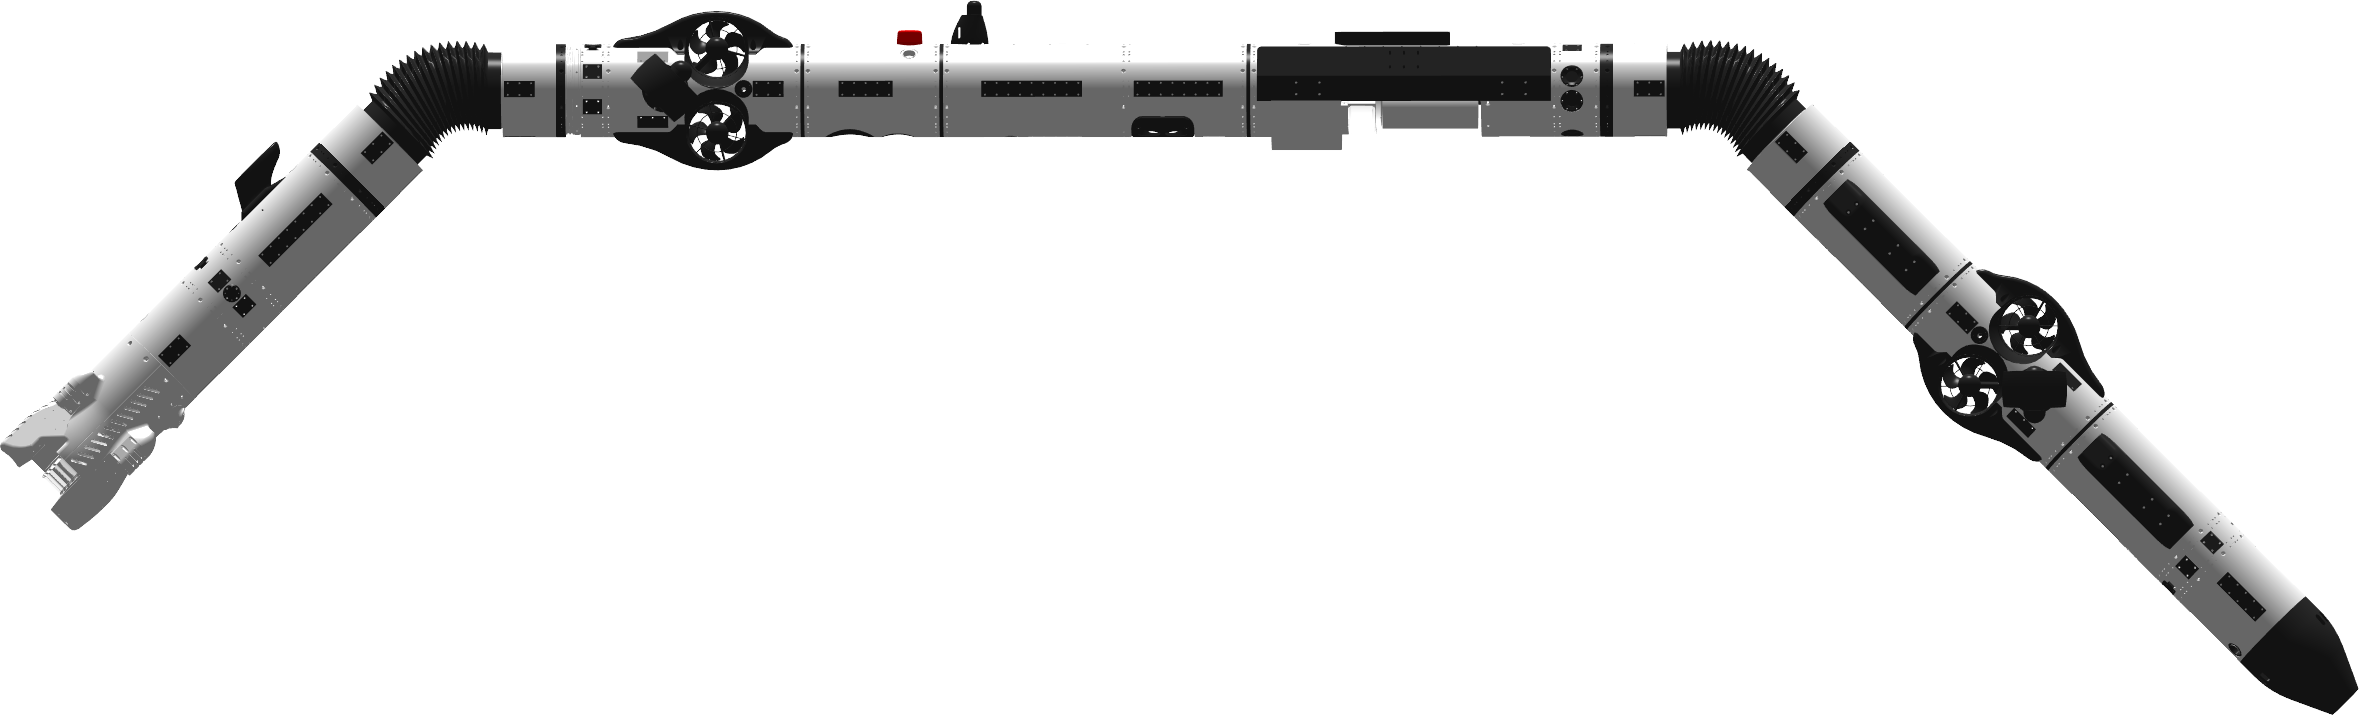
\includegraphics[width=\textwidth]{assets/side-view-45-joints.png}
    \caption{Image of Eelume robot in initial position for case \textit{stretch}}
    \label{fig:eelume:tpc:tasks:stretch:initial_pos}
\end{figure}

\begin{figure}[!ht]
    \centering
    \includegraphics[width=\textwidth,page=1]{assets/ignored/plots/tasks.pdf}
    \caption{Task trajectories for case \textit{stretch}.}
    \label{fig:eelume:tpc:tasks:stretch}
\end{figure}

The controller used for this group is the velocity-level task-pirority controller
presented in \autoref{sec:velocity_level_control}. The null-space projection method
is the augmented null-space projection method, and no damping of the jacobians
are used. The controller can be summarized in the following equation:
\begin{subequations}
\begin{align}
    \bm{\zeta}_d &= \sum_{i=1}^{3} \bm{N}_{i} \bm{J}_i^{+} \left( \dot{\bm{\sigma}}_{i,d} - \bm{\Lambda}_i \tilde{\bm{\sigma}}_i\right)  &
    \bm{\xi}_d &= \int_0^t \bm{J}_q(\bm{q}_b^n)\bm{\zeta}_d(\tau) \, d\tau + \bm{\xi}_0,
\end{align}
\end{subequations}
where the desired generalized state \(\bm{\xi}_d\)and desired generalized velocity
are used to set the references for the lower-level \gls{pd+} controller. The dependency
of time is implicit in the notation.

The task gains are set to diagonal matrices with the following values:
\begin{align}
    \bm{\Lambda}_1 &= 0.1 \I &
    \bm{\Lambda}_2 &= 0.1 \I &
    \bm{\Lambda}_3 &= 0.2 \I.
\end{align}

\begin{figure}[!ht]
    \centering
    \includegraphics[width=1.0\textwidth,page=3]{assets/ignored/plots/20250519-141527.pdf}
    \caption[Low-pass filtered position of Eelume robot during \textit{stretch} case with \gls{tpc}]
    {Low-pass filtered position of Eelume robot during \textit{stretch}. The position is offset from \((11, 36, 10)\)}
    \label{fig:results:tpc:stretch:1:pos}
\end{figure}
\begin{figure}[!ht]
    \centering
    \includegraphics[width=1.0\textwidth,page=4]{assets/ignored/plots/20250519-141527.pdf}
    \caption{Low-pass filtered generalized velocity of Eelume robot during \textit{stretch}}
    \label{fig:results:tpc:stretch:1:vel}
\end{figure}
\begin{figure}[!ht]
    \centering
    \includegraphics[width=1.0\textwidth,page=6]{assets/ignored/plots/20250519-141527.pdf}
    \caption{Desired body fixed forces, body-fixed momens and joint moments during case \textit{stretch}}
    \label{fig:results:tpc:stretch:1:forces}
\end{figure}
\begin{figure}[!ht]
    \centering
    \includegraphics[width=1.0\textwidth,page=5]{assets/ignored/plots/20250519-141527.pdf}
    \caption{Thruster and joint motor forces of during case \textit{stretch}}
    \label{fig:results:tpc:stretch:1:forces-torques}
\end{figure}
\begin{figure}[!ht]
    \centering
    \includegraphics[width=1.0\textwidth,page=7]{assets/ignored/plots/20250519-141527.pdf}
    \caption{Tail task value and error during case \textit{stretch}}
    \label{fig:results:tpc:stretch:1:task:1}
\end{figure}
\begin{figure}[!ht]
    \centering
    \includegraphics[width=1.0\textwidth,page=8]{assets/ignored/plots/20250519-141527.pdf}
    \caption{Head task value and error during case \textit{stretch}}
    \label{fig:results:tpc:stretch:1:task:2}
\end{figure}
\begin{figure}[!ht]
    \centering
    \includegraphics[width=1.0\textwidth,page=9]{assets/ignored/plots/20250519-141527.pdf}
    \caption{Body orientation task value and error during case \textit{stretch}}
    \label{fig:results:tpc:stretch:1:task:3}
\end{figure}
\begin{figure}[!ht]
    \centering
    \includegraphics[width=\textwidth,page=3]{assets/ignored/plots/tasks.pdf}
    \caption{Trajectory showing head- and tail-task values during case \textit{stretch}}
    \label{fig:results:tpc:stretch:task-traj}
\end{figure}
\begin{figure}[!ht]
    \centering
    \includegraphics[width=1.0\textwidth,page=11]{assets/ignored/plots/20250519-141527.pdf}
    \caption{Body orientation task value and error during case \textit{stretch}}
    \label{fig:results:tpc:stretch:dp-tracking}
\end{figure}



\iffalse
\paragraph{Results.}
\begin{itemize}
    \item \autoref{fig:results:tpc:stretch:1:pos} shows the position and orientation, as well as the joint angles, of the body link during the run. Note that the joint angles are lowpass filtered to try and remove some of the jittering as described in previous chapters 
    \item Most of the values look smooth, except for some oscillations of about 0.7 Hz with amplitude of about 1.5 degrees in roll
    \item There also seem to be some oscillation in the joint angles at about the same frequency and appriximately same amplitude. This is most noticeable on the second and fourth joint, bending about the \(z\)-axis.
    \item \autoref{fig:results:tpc:stretch:1:vel} shows the linear-, angular- and joint-velocities. The osciallation is more prominant here, and one can see some oscillation on the linear velocities as well.
    \item The frequency contents of all the velocity measurements seem to be at 0.6 - 0.8 Hz
    \item The lower-level \gls{pd+} controller commands the body fixed wrench and joint torques shown in \autoref{fig:results:tpc:stretch:1:forces} where some of the same oscillatory behaviour as for the generalized position plot is shown.
    \item \autoref{fig:results:tpc:stretch:1:forces-torques} shows the commanded thruster forces and joint motor moments. It is observed that they
        are all oscillatory with approximately the same frequency as the other plots.
    \item \autoref{fig:results:tpc:stretch:1:task:1} Shows the task value and error for the tail task, the highest priority tasks. It is observed
        that at time 0 the position is about \(80\) cm off the desired tail position, but it slowly converges towards 0 these 20 seconds. Throughout the run the task error keeps a low value of about \(20\) cm off, but settles to approximately \(10\) cm after 45 seconds.
    \item \autoref{fig:results:tpc:stretch:1:task:2} shows the task 2 error (head task). For thus run there is some initial error, which is partially corrected during the first 20 seconds. In the period between 20 and 40 seconds the error seems to be better, being less than 10 cm off for a couple of seconds. After 40 seconds the error raises in an appriximately linear fashion.
    \item \autoref{fig:results:tpc:stretch:1:task:3} shows the orientation task. The error for this task is low all throughout the run, meaning the body
        was able to be aligned with the inertial frame withougt large deviations all throught the run.
    \item \autoref{fig:results:tpc:stretch:task-traj} shows the head and tail task trajectories in the north-down plane.    One can see that the tail task follows the desired task trajectory wel. The head error starts around the ference, but eventually goes south. The position of the body moves down and south.
    \item \autoref{fig:results:tpc:stretch:dp-tracking} shows how ell the lower-level \gls{pd+} controller tracks the reference set by the task-priority controller. We see that it is very good for the position and joint agles, but the orientation tracking is a bit slow. 
\end{itemize}

\paragraph{Discussion.}
\begin{itemize}
    \item oscillations on joints can be from low-pass filtering of the joint angles and generalized velocities. Low-pass filtering of the joint measurements are fed into the controller, which can typically cause some oscillatory behaviour, especially. It is hard to say if this is the case.
    \item Low-pass filtering is a tradeoff: removing noise will introduce time delays. This tradeoff is discussed more in-depth in \autoref{sec:results:lowpass}. 
    \item It should also be noted that \atoref{fig:results:tpc:stretch:1:forces-torques}, are not the actual measured thruster forces and joint moment measurements, but rather the setpoints for lower-level controllers on the Eelume robot. There are time-delays in this part of the system that is partly unknown and can contribute to time dealays causing oscillations.
    \item A possible explanation can also be the interaction with the controller gains in the higher-level task-priority controller with the lower-level \gls{pd+} controller. If the lower-level controller is aggressive, and the proportional gain in the task-priority controller is large we might expect some oscilation in the reference. We can however dismiss this explanation seeing the smoothness of the reference in \autoref{fig:results:tpc:stretch:dp-tracking}.
    \item The first 20 seconds the tpc controller has no feed-farward term from the desired task velocity, meaning the response is drived by the task error being integrated up as \(\bm{\xi}_d\). For the tail and head tasks: it is still able to converge to about \(20\) cm from the desired tail and head position the first \(20\) seconds. 
    \item Task 1 error and task 2 error. after the first 20 seconds, we see that the two position taks are low. When the robot stretches out, task 2 error increases. We also expect a linear increase in the task 2 error because the head task moves linearly south.
    \item why is orientation tracking slow? The third task is orientation, it has low priority. We expect the higher order tasks to want to change the orientation, especially the pitch to better track the desired positions.
    \item All in all as expected, have demonstated the piroirty of the tasks, a good tracking of both tasks is observed when it is possible to track both task, when is becomes impossible due to kinematic constrints, the task with the highest priority actually takes priority.
\end{itemize}

\fi

\paragraph{Results.}

\autoref{fig:results:tpc:stretch:1:pos} shows the position, orientation, and joint angles of the Eelume robot during the task-priority control experiment. To mitigate the measurement noise described in previous sections, the joint angle signals are low-pass filtered. Most values appear smooth, although a mild oscillation with a frequency of approximately \(0.7\,\mathrm{Hz}\) and amplitude around \(1.5^\circ\) is noticeable in the roll angle. Similar oscillations are also observed in the second and fourth joint angles, which primarily rotate about the \(z\)-axis.

These oscillations are more pronounced in the velocity signals shown in \autoref{fig:results:tpc:stretch:1:vel}, which includes linear, angular, and joint velocities. The dominant frequency content across all velocity signals lies between \(0.6\) and \(0.8\,\mathrm{Hz}\).

\autoref{fig:results:tpc:stretch:1:forces} displays the body-fixed wrench and joint torques commanded by the lower-level \gls{pd+} controller. Oscillatory behavior is again evident, reflecting the dynamics seen in the position and velocity data. This is further confirmed in \autoref{fig:results:tpc:stretch:1:forces-torques}, which shows the commanded thruster forces and joint motor torques, both of which exhibit similar frequency characteristics.

Task-specific performance is visualized in \autoref{fig:results:tpc:stretch:1:task:1} and \ref{fig:results:tpc:stretch:1:task:3}. The highest priority task (tail position) begins with an initial error of approximately \(80\,\mathrm{cm}\), which gradually reduces during the first \(20\) seconds. The error stabilizes around \(20\,\mathrm{cm}\) for most of the run and settles close to \(10\,\mathrm{cm}\) after \(45\) seconds.

The second task (head position) shows partial correction of the initial error within the first \(20\) seconds, as seen in \autoref{fig:results:tpc:stretch:1:task:2}. Between \(t = 20\) and \(40\,\mathrm{s}\), the error remains below \(10\,\mathrm{cm}\), but then increases approximately linearly—consistent with the desired trajectory for the head task, which continues to move south.

\autoref{fig:results:tpc:stretch:1:task:3} shows the orientation task (lowest priority). The error remains small throughout the run, indicating successful alignment of the robot body with the inertial frame, though with slower tracking compared to position tasks.

Task-space trajectories for the head and tail tasks in the north-down plane are shown in \autoref{fig:results:tpc:stretch:task-traj}. The tail closely follows its reference trajectory, while the head initially follows but diverges later, moving south as expected. This movement corresponds to the overall body trajectory.

\autoref{fig:results:tpc:stretch:dp-tracking} demonstrates how well the lower-level \gls{pd+} controller tracks the reference commands from the task-priority controller. Position and joint angle tracking are accurate, while orientation tracking appears slightly delayed.

\paragraph{Discussion.}

The observed oscillations in roll and joint angles may originate from the use of low-pass filtered signals for feedback. Filtering helps suppress noise but introduces phase delay, which can lead to oscillatory behavior, particularly when feedback loops interact with higher-frequency signal components. This trade-off is further discussed in \autoref{sec:results:lowpass}.

It is important to note that the plots in \autoref{fig:results:tpc:stretch:1:forces-torques} reflect **commanded** values to the low-level controllers—not the actual measured forces or torques. Time delays inherent in the actuation system—some of which are unmodeled—can contribute to oscillatory or delayed responses in the physical system.

Another possible cause of oscillations is interaction between the task-priority controller and the lower-level \gls{pd+} controller. However, the smoothness of the tracked references in \autoref{fig:results:tpc:stretch:dp-tracking} suggests that this interaction is not problematic in this case.

During the first \(20\) seconds, the task-priority controller does not use a feedforward term from the desired task velocity, meaning the system relies solely on accumulated task error to generate motion. Despite this, the controller successfully reduces the tail and head task errors to within \(20\,\mathrm{cm}\), demonstrating effective control.

After the initial transient, both task errors remain low. However, as the robot stretches out and the head reference continues to move south, the head task error increases. This is expected, as task-priority control respects task hierarchy: when it becomes kinematically infeasible to satisfy all objectives simultaneously, the lower-priority task (head position) is sacrificed in favor of the higher-priority task (tail position).

The slower response in orientation tracking is also expected, given that orientation is the third-priority task. As the robot aligns its body to meet the position tasks, it may need to adjust its pitch, thereby introducing a delay in satisfying the orientation objective.

In summary, the experiment demonstrates that task-priority control operates as intended. When multiple tasks are simultaneously feasible, all are tracked accurately. When constraints make full satisfaction impossible, higher-priority tasks dominate—consistent with theoretical expectations of task-priority frameworks.


\FloatBarrier

% -----------------------------------------------------------------------------
\newpage
\section{Velocity-Level \gls{tpc}, case \textit{bend}}

\paragraph{Experimental setup}
The third group of experiments aims to show the performance of the set-based
velocity-level task-priority controller. This controller is used to set
joint limits of \(\pm 45\) degrees on the \(y\)-axis joints. The task setup is,
excluding the set-based tasks:
\begin{enumerate}
    \item \(\bm{\sigma}_1(\bm{\xi}) \in \R^3\): The position of the tail. Moving downwards and forwards.
    \item \(\bm{\sigma}_2(\bm{\xi}) \in \R^3\): The position of the head. Moving downwards and backwards.
    \item \(\bm{\sigma}_3(\bm{\xi}) \in \R^3\): The attitude of the base link. Set to have the same orientation as the inertial frame.
\end{enumerate}
\autoref{fig:eelume:tpc:tasks:bend} shows an overview of the tasks. Notice how
the position of the head and the tail close each other as the time increases, meaning
that the joints will have to bend to keep the tasks fullfilled. This means
that the joint limits will become active at some point during the run. Because
of the nature of the experiment, this case is referred to as \textit{bend}.
The controller
used for this group is the same as for the previous group, but with the set-based
tasks taking priority over the position and attitude tasks when thay are activated.

\begin{figure}[!ht]
    \centering
    \includegraphics[width=\textwidth,page=2]{assets/ignored/plots/tasks.pdf}
    \caption{Overview of head and tail tasks for case \textit{bend}.}
    \label{fig:eelume:tpc:tasks:bend}
\end{figure}

\paragraph{Results.}

\begin{figure}[!ht]
    \centering
    \includegraphics[width=\textwidth,page=4]{assets/ignored/plots/tasks.pdf}
    \caption{Trajectory showing head- and tail-task values during case \textit{bend}}
    \label{fig:results:tpc:bend:task-traj}
\end{figure}
\begin{figure}[!ht]
    \centering
    \includegraphics[width=\textwidth,page=5]{assets/ignored/plots/tasks.pdf}
    \caption{Comparison of task errors for case \textit{bend}}
    \label{fig:results:tpc:bend:task-errors}
\end{figure}

\begin{figure}[!ht]
    \centering
    \includegraphics[width=1.0\textwidth,page=3]{assets/ignored/plots/20250519-161629.pdf}
    \caption[Low-pass filtered position of Eelume robot during \textit{stretch} case with \gls{tpc}]
    {Low-pass filtered position of Eelume robot during \textit{stretch}. The position is offset from \((11, 36, 10)\)}
    \label{fig:results:tpc:bend:1:pos}
\end{figure}
\begin{figure}[!ht]
    \centering
    \includegraphics[width=1.0\textwidth,page=5]{assets/ignored/plots/20250519-161629.pdf}
    \caption{Thruster and joint motor forces of during case \textit{bend}}
    \label{fig:results:tpc:bend:1:forces-torques}
\end{figure}

\begin{figure}[!ht]
    \centering
    \includegraphics[width=1.0\textwidth,page=11]{assets/ignored/plots/20250519-161629.pdf}
    \caption{Body orientation task value and error during case \textit{bend}}
    \label{fig:results:tpc:bend:dp-tracking}
\end{figure}



\autoref{fig:results:tpc:bend:task-traj} shows the trajectories of the head and tail tasks in the north-down plane. Initially, both tasks are tracked reasonably well. However, after approximately 25 seconds, a divergence from the desired trajectories is observed. Specifically, the head and tail depths begin to decrease, deviating from the planned paths. This trend is also visible in the overall body trajectory, shown in black, which ascends after the same time point.

This behavior is further supported by the task error plots shown in \autoref{fig:results:tpc:bend:task-errors}, which present the error evolution for the head, tail, and orientation tasks. For the first 25 seconds, the task errors remain within acceptable bounds. Beyond this point, the head and tail errors increase approximately linearly, indicating a loss of accurate tracking. Meanwhile, the orientation task remains well-regulated throughout the run, with consistently low error.

\autoref{fig:results:tpc:bend:1:pos} presents the full pose and joint angle history for the experiment. The position data is generally smooth, with the downward drift in depth after the 25-second mark matching the observations in the task trajectories. Notably, this time corresponds with the activation of set-based constraints, as the first and third joint angles reach their lower limits. These joints subsequently stabilize, oscillating slightly within the range of approximately \([-50^\circ, -45^\circ]\).

Minor oscillations are also observed in the orientation data, particularly in the roll angle. These oscillations occur at a frequency of about \(0.7\,\mathrm{Hz}\) and have an amplitude of roughly \(1.5^\circ\).

The actuator commands during the run are shown in \autoref{fig:results:tpc:bend:1:forces-torques}. Oscillations in both thruster forces and joint torques become more pronounced after 15 seconds. \autoref{fig:results:tpc:bend:dp-tracking} compares the reference and actual generalized positions. As the joint limits are reached, the reference velocities for joints 1 and 3 flatten out, indicating saturation due to the active joint constraints. Furthermore, while the controller tracks the east and depth references reasonably well, it struggles to maintain accuracy in the north direction.

\paragraph{Discussion.}

The key question arising from this experiment is why the robot begins to deviate from the task trajectories—specifically, why it reduces depth after 25 seconds. The data strongly suggests that this behavior coincides with activation of the joint limit constraints, as indicated in \autoref{fig:results:tpc:bend:1:pos}. Once the first and third joints hit their limits, the associated set-based tasks are activated and assigned higher priority than the head, tail, and orientation tasks.

The task Jacobian associated with the joint limit constraint for \(\theta_1\) is a \(1 \times 10\) row vector with all zeros except for a single one in the seventh position:
\[
\bm{J}_s = [0\ 0\ 0\ 0\ 0\ 0\ 1\ 0\ 0\ 0].
\]
This structure reflects the fact that the task directly constrains only \(\theta_1\), with no influence from other generalized coordinates. The corresponding null-space projector \(\bm{N}_s = \I - \bm{J}_s^{+} \bm{J}_s\) is thus nearly the identity matrix, except for a zero in the position corresponding to \(\theta_1\):
\begin{align}
\bm{N}_s = 
\begin{bmatrix}
1 &   &        &        &  \\
  & \ddots &        &        & \\
  &   & 0      &        &\\
  &   &        & \ddots      & \\
  &   &        &        & 1
\end{bmatrix}.
\end{align}

This null-space projector effectively zeroes out the component of the desired generalized velocity \(\bm{\zeta}_d\) that corresponds to motion in \(\theta_1\). As a result, when the set-based task is activated, it overrides any previously computed joint velocity in that direction. The full control law becomes:
\begin{align}
    \bm{\zeta}_d = \bm{J}_s^{+}\bm{\Lambda}_s \tilde{\bm{\sigma}}_s + \bm{N}_s \sum_{i=1}^k \bm{N}_i^{\#}\bm{J}_i^{\#} \left(\dot{\bm{\sigma}}_{i,d} + \bm{\Lambda}_i \tilde{\bm{\sigma}}_i\right),
\end{align}
which ensures that the constraint is enforced at the cost of suppressing any conflicting joint motion from lower-priority tasks.

One can imagine that, in the absence of joint limits, the controller would command the robot to ascend (decrease depth) while bending the joints to maintain head and tail positions. However, once the joint motions are blocked by the set-based constraints, the required joint contributions to those tasks cannot be realized. As a result, the controller instead produces a net upward base motion, leading to the observed depth reduction.

This interpretation is further supported by the data in \autoref{fig:results:tpc:bend:dp-tracking}, which shows that the reference depth itself decreases—indicating that the behavior originates from the controller’s task prioritization rather than a failure of the low-level depth regulation.

In summary, this experiment highlights a fundamental limitation of task-priority control when using set-based tasks. While the method correctly enforces constraints, it can result in undesired behavior if task interactions are not carefully considered. Designing compatible and non-conflicting tasks is therefore essential for reliable system behavior.

\FloatBarrier


% -----------------------------------------------------------------------------
\newpage
\section{Low-Pass Filtering}
\label{sec:results:lowpass_filtering}
\label{sec:results:lowpass}

\paragraph{Experimental setup.}
This group of experiments aim to show the effects of low-pass filtering the
joint angles and velocity measurments. To do this, the same scenario as in \autoref{sec:res:stretch}, case \textit{stretch},
are run. One run low-pass filter the joint angles and the other passes the measurements
directly to the controller without filtering them. The two cases are reffered to as:
\begin{itemize}
    \item \textit{filter}. A velocity-level \gls{tpc} run with low-pass filtering of joint angles and generalized velocities.
        Control loop frequency: \(50\) Hz.
    \item \textit{un-filtered}. A velocity-level \gls{tpc} run with no low-pass filtering of the states.
        Control loop frequency: \(100\) Hz.
\end{itemize}

\paragraph{Results}

\begin{figure}[h!]
    \centering
    \includegraphics[width=1.0\textwidth,page=1]{assets/ignored/plots/20250519-135739.pdf}
    \caption{Low-pass filtered position of the Eelume robot during case \textit{filter}}
    \label{fig:results:tpc:filter:pos}
\end{figure}
\begin{figure}[h!]
    \centering
    \includegraphics[width=1.0\textwidth,page=1]{assets/ignored/plots/20250513-154920.pdf}
    \caption{Position of the Eelume robot during case \textit{un-filtered}}
    \label{fig:results:tpc:un-filtered:pos}
\end{figure}
\begin{figure}[h!]
    \centering
    \includegraphics[width=1.0\textwidth,page=5]{assets/ignored/plots/20250519-135739.pdf}
    \caption{Allocated thruster forces and joint moment during case \textit{filter}}
    \label{fig:results:tpc:filter:forces}
\end{figure}
\begin{figure}[h!]
    \centering
    \includegraphics[width=1.0\textwidth,page=5]{assets/ignored/plots/20250513-154920.pdf}
    \caption{Allocated thruster forces and joint moment during case \textit{un-filtered}}
    \label{fig:results:tpc:un-filtered:forces}
\end{figure}
\begin{figure}[h!]
    \centering
    \includegraphics[width=1.0\textwidth,page=1]{assets/ignored/plots/tasks-filter.pdf}
    \caption{Comparison of task errors between cases \textit{filter} and \textit{un-filtered}}
    \label{fig:results:tpc:filter:task-errors}
\end{figure}

\autoref{fig:results:tpc:filter:pos} presents the position, orientation, and joint angles during the filtered run. The position trajectories appear smooth and continuous. The Euler angles, however, exhibit noticeable oscillations—particularly in the roll angle, where oscillations of approximately \(2^\circ\) amplitude occur at a frequency of around \(0.5\,\mathrm{Hz}\). Similar oscillations are present in the yaw angle, though with slightly lower amplitude. The pitch angle also contains some oscillatory behavior, but it is considerably less pronounced.

In contrast, \autoref{fig:results:tpc:un-filtered:pos} shows the same quantities for the unfiltered run. The position remains smooth, but the roll angle exhibits high-frequency noise, particularly during the first 30 seconds of the run. This noise has a frequency of around \(3\,\mathrm{Hz}\) and amplitude below \(1^\circ\). The pitch angle shows similar transient noise. Most notably, the joint angle signals—especially for joints 1 and 3—display strong jitter throughout the run. Nevertheless, aside from this jitter, the underlying joint trajectories remain smooth.

\autoref{fig:results:tpc:filter:forces} shows the commanded thruster forces and joint motor torques for the filtered case. Oscillations are present across all channels, with a consistent frequency of approximately \(0.5\,\mathrm{Hz}\), matching the dominant oscillatory behavior observed in the pose and joint signals. Although the signals are not noise-free, they are visibly smoother and more interpretable than those in the unfiltered case.

In \autoref{fig:results:tpc:un-filtered:forces}, the unfiltered case reveals highly jittery actuator signals. The thruster references are dominated by high-frequency noise, especially during the first 30 seconds, to the extent that the underlying signal is nearly obscured. Some reduction in jitter is seen as the experiment progresses. The joint motor torques repeatedly saturate at the \(\pm 16\,\mathrm{Nm}\) limit, resulting in behavior reminiscent of a "bang-bang" controller rather than smooth torque regulation.

\autoref{fig:results:tpc:filter:task-errors} compares the task errors for the filtered and unfiltered runs. In both cases, the tail and head task errors converge toward zero within the first 20 seconds, after which different behaviors emerge.

The tail task is better tracked in the unfiltered case, where the error remains within \(0.1\,\mathrm{m}\) for the final 15 seconds. In contrast, the filtered case shows a larger deviation, reaching over \(0.4\,\mathrm{m}\) during the same interval. Conversely, the head task exhibits more favorable tracking in the filtered run. While both cases show approximately linear growth in error after the robot stretches out, the filtered case maintains an error that is consistently more than \(0.2\,\mathrm{m}\) lower than in the unfiltered scenario.
The orientation task performs similarly in both runs, with low tracking error throughout the experiment.


\paragraph{Discussion}
The comparison between filtered and unfiltered sensor measurements reveals several important trade-offs in system performance and control signal quality.

First, there is evidence that low-pass filtering may induce low-frequency oscillations in the system. Oscillations around \(0.5\,\mathrm{Hz}\) are clearly visible in the position and orientation data when filtering is enabled, and similar oscillatory behavior is observed in the allocated thruster forces and joint moments. These patterns are not present in the unfiltered run. However, it is important to note that the filtered and unfiltered experiments were conducted with different control loop frequencies. Since the loop frequency influences the controller's bandwidth, it may also contribute to the observed oscillations, making it difficult to attribute them solely to filtering.

Despite the high-frequency jitter observed in the unfiltered case, the overall control performance appears acceptable. This can partly be explained by the behavior of the lower-level controllers, which act as implicit low-pass filters when tracking the setpoint references. Pre-filtering the measurements before they reach the low-level controllers may therefore suppress frequencies that the hardware could have followed. However, continuously commanding noisy, high-frequency signals can be damaging to physical actuators, particularly joint motors, which are sensitive to rapid switching and saturation.

When comparing the actuator signals in both cases, a clear trade-off becomes evident. Without filtering, the joint moments and body-fixed torques exhibit high-frequency noise, especially during the early stages of the run. With filtering, these inputs are much smoother overall, although they show low-frequency oscillations around \(0.5\,\mathrm{Hz}\). Evaluating controller performance through task error plots in \autoref{fig:results:tpc:filter:task-errors} does not clearly favor one approach over the other; both cases exhibit strengths and weaknesses depending on the specific task and phase of motion.

Considering the risk of hardware degradation due to persistent high-frequency input signals, it may be advisable to apply low-pass filtering, despite the induced oscillations. Further tuning of the filter parameters and additional experiments are needed to identify a better compromise between signal smoothness and control responsiveness.






